
%% bare_conf.tex
%% V1.3
%% 2007/01/11
%% by Michael Shell
%% See:
%% http://www.michaelshell.org/
%% for current contact information.
%%
%% This is a skeleton file demonstrating the use of IEEEtran.cls
%% (requires IEEEtran.cls version 1.7 or later) with an IEEE conference paper.
%%
%% Support sites:
%% http://www.michaelshell.org/tex/ieeetran/
%% http://www.ctan.org/tex-archive/macros/latex/contrib/IEEEtran/
%% and
%% http://www.ieee.org/

%%*************************************************************************
%% Legal Notice:
%% This code is offered as-is without any warranty either expressed or
%% implied; without even the implied warranty of MERCHANTABILITY or
%% FITNESS FOR A PARTICULAR PURPOSE! 
%% User assumes all risk.
%% In no event shall IEEE or any contributor to this code be liable for
%% any damages or losses, including, but not limited to, incidental,
%% consequential, or any other damages, resulting from the use or misuse
%% of any information contained here.
%%
%% All comments are the opinions of their respective authors and are not
%% necessarily endorsed by the IEEE.
%%
%% This work is distributed under the LaTeX Project Public License (LPPL)
%% ( http://www.latex-project.org/ ) version 1.3, and may be freely used,
%% distributed and modified. A copy of the LPPL, version 1.3, is included
%% in the base LaTeX documentation of all distributions of LaTeX released
%% 2003/12/01 or later.
%% Retain all contribution notices and credits.
%% ** Modified files should be clearly indicated as such, including  **
%% ** renaming them and changing author support contact information. **
%%
%% File list of work: IEEEtran.cls, IEEEtran_HOWTO.pdf, bare_adv.tex,
%%                    bare_conf.tex, bare_jrnl.tex, bare_jrnl_compsoc.tex
%%*************************************************************************

% *** Authors should verify (and, if needed, correct) their LaTeX system  ***
% *** with the testflow diagnostic prior to trusting their LaTeX platform ***
% *** with production work. IEEE's font choices can trigger bugs that do  ***
% *** not appear when using other class files.                            ***
% The testflow support page is at:
% http://www.michaelshell.org/tex/testflow/



% Note that the a4paper option is mainly intended so that authors in
% countries using A4 can easily print to A4 and see how their papers will
% look in print - the typesetting of the document will not typically be
% affected with changes in paper size (but the bottom and side margins will).
% Use the testflow package mentioned above to verify correct handling of
% both paper sizes by the user's LaTeX system.
%
% Also note that the "draftcls" or "draftclsnofoot", not "draft", option
% should be used if it is desired that the figures are to be displayed in
% draft mode.
%
\documentclass[conference]{IEEEtran}
% Add the compsoc option for Computer Society conferences.
%
% If IEEEtran.cls has not been installed into the LaTeX system files,
% manually specify the path to it like:
% \documentclass[conference]{../sty/IEEEtran}





% Some very useful LaTeX packages include:
% (uncomment the ones you want to load)


% *** MISC UTILITY PACKAGES ***
%
%\usepackage{ifpdf}
% Heiko Oberdiek's ifpdf.sty is very useful if you need conditional
% compilation based on whether the output is pdf or dvi.
% usage:
% \ifpdf
%   % pdf code
% \else
%   % dvi code
% \fi
% The latest version of ifpdf.sty can be obtained from:
% http://www.ctan.org/tex-archive/macros/latex/contrib/oberdiek/
% Also, note that IEEEtran.cls V1.7 and later provides a builtin
% \ifCLASSINFOpdf conditional that works the same way.
% When switching from latex to pdflatex and vice-versa, the compiler may
% have to be run twice to clear warning/error messages.






% *** CITATION PACKAGES ***
%
\usepackage{cite}
\usepackage{array}
\usepackage{booktabs}
\usepackage[]{subfigure}
% cite.sty was written by Donald Arseneau
% V1.6 and later of IEEEtran pre-defines the format of the cite.sty package
% \cite{} output to follow that of IEEE. Loading the cite package will
% result in citation numbers being automatically sorted and properly
% "compressed/ranged". e.g., [1], [9], [2], [7], [5], [6] without using
% cite.sty will become [1], [2], [5]--[7], [9] using cite.sty. cite.sty's
% \cite will automatically add leading space, if needed. Use cite.sty's
% noadjust option (cite.sty V3.8 and later) if you want to turn this off.
% cite.sty is already installed on most LaTeX systems. Be sure and use
% version 4.0 (2003-05-27) and later if using hyperref.sty. cite.sty does
% not currently provide for hyperlinked citations.
% The latest version can be obtained at:
% http://www.ctan.org/tex-archive/macros/latex/contrib/cite/
% The documentation is contained in the cite.sty file itself.






% *** GRAPHICS RELATED PACKAGES ***
%
\usepackage{graphicx}
\ifCLASSINFOpdf
  % \usepackage[pdftex]{graphicx}
  % declare the path(s) where your graphic files are
  % \graphicspath{{../pdf/}{../jpeg/}}
  % and their extensions so you won't have to specify these with
  % every instance of \includegraphics
  % \DeclareGraphicsExtensions{.pdf,.jpeg,.png}
\else
  % or other class option (dvipsone, dvipdf, if not using dvips). graphicx
  % will default to the driver specified in the system graphics.cfg if no
  % driver is specified.
  % \usepackage[dvips]{graphicx}
  % declare the path(s) where your graphic files are
  % \graphicspath{{../eps/}}
  % and their extensions so you won't have to specify these with
  % every instance of \includegraphics
  % \DeclareGraphicsExtensions{.eps}
\fi
% graphicx was written by David Carlisle and Sebastian Rahtz. It is
% required if you want graphics, photos, etc. graphicx.sty is already
% installed on most LaTeX systems. The latest version and documentation can
% be obtained at: 
% http://www.ctan.org/tex-archive/macros/latex/required/graphics/
% Another good source of documentation is "Using Imported Graphics in
% LaTeX2e" by Keith Reckdahl which can be found as epslatex.ps or
% epslatex.pdf at: http://www.ctan.org/tex-archive/info/
%
% latex, and pdflatex in dvi mode, support graphics in encapsulated
% postscript (.eps) format. pdflatex in pdf mode supports graphics
% in .pdf, .jpeg, .png and .mps (metapost) formats. Users should ensure
% that all non-photo figures use a vector format (.eps, .pdf, .mps) and
% not a bitmapped formats (.jpeg, .png). IEEE frowns on bitmapped formats
% which can result in "jaggedy"/blurry rendering of lines and letters as
% well as large increases in file sizes.
%
% You can find documentation about the pdfTeX application at:
% http://www.tug.org/applications/pdftex





% *** MATH PACKAGES ***
%
\usepackage[cmex10]{amsmath}
% A popular package from the American Mathematical Society that provides
% many useful and powerful commands for dealing with mathematics. If using
% it, be sure to load this package with the cmex10 option to ensure that
% only type 1 fonts will utilized at all point sizes. Without this option,
% it is possible that some math symbols, particularly those within
% footnotes, will be rendered in bitmap form which will result in a
% document that can not be IEEE Xplore compliant!
%
% Also, note that the amsmath package sets \interdisplaylinepenalty to 10000
% thus preventing page breaks from occurring within multiline equations. Use:
%\interdisplaylinepenalty=2500
% after loading amsmath to restore such page breaks as IEEEtran.cls normally
% does. amsmath.sty is already installed on most LaTeX systems. The latest
% version and documentation can be obtained at:
% http://www.ctan.org/tex-archive/macros/latex/required/amslatex/math/





% *** SPECIALIZED LIST PACKAGES ***
%
%\usepackage{algorithmic}
% algorithmic.sty was written by Peter Williams and Rogerio Brito.
% This package provides an algorithmic environment fo describing algorithms.
% You can use the algorithmic environment in-text or within a figure
% environment to provide for a floating algorithm. Do NOT use the algorithm
% floating environment provided by algorithm.sty (by the same authors) or
% algorithm2e.sty (by Christophe Fiorio) as IEEE does not use dedicated
% algorithm float types and packages that provide these will not provide
% correct IEEE style captions. The latest version and documentation of
% algorithmic.sty can be obtained at:
% http://www.ctan.org/tex-archive/macros/latex/contrib/algorithms/
% There is also a support site at:
% http://algorithms.berlios.de/index.html
% Also of interest may be the (relatively newer and more customizable)
% algorithmicx.sty package by Szasz Janos:
% http://www.ctan.org/tex-archive/macros/latex/contrib/algorithmicx/




% *** ALIGNMENT PACKAGES ***
%
%\usepackage{array}
% Frank Mittelbach's and David Carlisle's array.sty patches and improves
% the standard LaTeX2e array and tabular environments to provide better
% appearance and additional user controls. As the default LaTeX2e table
% generation code is lacking to the point of almost being broken with
% respect to the quality of the end results, all users are strongly
% advised to use an enhanced (at the very least that provided by array.sty)
% set of table tools. array.sty is already installed on most systems. The
% latest version and documentation can be obtained at:
% http://www.ctan.org/tex-archive/macros/latex/required/tools/


%\usepackage{mdwmath}
%\usepackage{mdwtab}
% Also highly recommended is Mark Wooding's extremely powerful MDW tools,
% especially mdwmath.sty and mdwtab.sty which are used to format equations
% and tables, respectively. The MDWtools set is already installed on most
% LaTeX systems. The lastest version and documentation is available at:
% http://www.ctan.org/tex-archive/macros/latex/contrib/mdwtools/


% IEEEtran contains the IEEEeqnarray family of commands that can be used to
% generate multiline equations as well as matrices, tables, etc., of high
% quality.


%\usepackage{eqparbox}
% Also of notable interest is Scott Pakin's eqparbox package for creating
% (automatically sized) equal width boxes - aka "natural width parboxes".
% Available at:
% http://www.ctan.org/tex-archive/macros/latex/contrib/eqparbox/





% *** SUBFIGURE PACKAGES ***
%\usepackage[tight,footnotesize]{subfigure}
% subfigure.sty was written by Steven Douglas Cochran. This package makes it
% easy to put subfigures in your figures. e.g., "Figure 1a and 1b". For IEEE
% work, it is a good idea to load it with the tight package option to reduce
% the amount of white space around the subfigures. subfigure.sty is already
% installed on most LaTeX systems. The latest version and documentation can
% be obtained at:
% http://www.ctan.org/tex-archive/obsolete/macros/latex/contrib/subfigure/
% subfigure.sty has been superceeded by subfig.sty.



%\usepackage[caption=false]{caption}
%\usepackage[font=footnotesize]{subfig}
% subfig.sty, also written by Steven Douglas Cochran, is the modern
% replacement for subfigure.sty. However, subfig.sty requires and
% automatically loads Axel Sommerfeldt's caption.sty which will override
% IEEEtran.cls handling of captions and this will result in nonIEEE style
% figure/table captions. To prevent this problem, be sure and preload
% caption.sty with its "caption=false" package option. This is will preserve
% IEEEtran.cls handing of captions. Version 1.3 (2005/06/28) and later 
% (recommended due to many improvements over 1.2) of subfig.sty supports
% the caption=false option directly:
%\usepackage[caption=false,font=footnotesize]{subfig}
%
% The latest version and documentation can be obtained at:
% http://www.ctan.org/tex-archive/macros/latex/contrib/subfig/
% The latest version and documentation of caption.sty can be obtained at:
% http://www.ctan.org/tex-archive/macros/latex/contrib/caption/




% *** FLOAT PACKAGES ***
%
%\usepackage{fixltx2e}
% fixltx2e, the successor to the earlier fix2col.sty, was written by
% Frank Mittelbach and David Carlisle. This package corrects a few problems
% in the LaTeX2e kernel, the most notable of which is that in current
% LaTeX2e releases, the ordering of single and double column floats is not
% guaranteed to be preserved. Thus, an unpatched LaTeX2e can allow a
% single column figure to be placed prior to an earlier double column
% figure. The latest version and documentation can be found at:
% http://www.ctan.org/tex-archive/macros/latex/base/



%\usepackage{stfloats}
% stfloats.sty was written by Sigitas Tolusis. This package gives LaTeX2e
% the ability to do double column floats at the bottom of the page as well
% as the top. (e.g., "\begin{figure*}[!b]" is not normally possible in
% LaTeX2e). It also provides a command:
%\fnbelowfloat
% to enable the placement of footnotes below bottom floats (the standard
% LaTeX2e kernel puts them above bottom floats). This is an invasive package
% which rewrites many portions of the LaTeX2e float routines. It may not work
% with other packages that modify the LaTeX2e float routines. The latest
% version and documentation can be obtained at:
% http://www.ctan.org/tex-archive/macros/latex/contrib/sttools/
% Documentation is contained in the stfloats.sty comments as well as in the
% presfull.pdf file. Do not use the stfloats baselinefloat ability as IEEE
% does not allow \baselineskip to stretch. Authors submitting work to the
% IEEE should note that IEEE rarely uses double column equations and
% that authors should try to avoid such use. Do not be tempted to use the
% cuted.sty or midfloat.sty packages (also by Sigitas Tolusis) as IEEE does
% not format its papers in such ways.





% *** PDF, URL AND HYPERLINK PACKAGES ***
%
%\usepackage{url}
% url.sty was written by Donald Arseneau. It provides better support for
% handling and breaking URLs. url.sty is already installed on most LaTeX
% systems. The latest version can be obtained at:
% http://www.ctan.org/tex-archive/macros/latex/contrib/misc/
% Read the url.sty source comments for usage information. Basically,
% \url{my_url_here}.





% *** Do not adjust lengths that control margins, column widths, etc. ***
% *** Do not use packages that alter fonts (such as pslatex).         ***
% There should be no need to do such things with IEEEtran.cls V1.6 and later.
% (Unless specifically asked to do so by the journal or conference you plan
% to submit to, of course. )


% correct bad hyphenation here
\hyphenation{op-tical net-works semi-conduc-tor}


\begin{document}
%
% paper title
% can use linebreaks \\ within to get better formatting as desired
\title{Functional Connectivity from EEG Signals during Perceiving Pleasant and Unpleasant Odors}


% author names and affiliations
% use a multiple column layout for up to three different
% affiliations
%\author{
%\IEEEauthorblockN{He Xu}
%\IEEEauthorblockA{Multimedia Signal Processing\\ Group, EPFL\\
%Lausanne, Switzerland\\
%he.xu@epfl.ch}
%
%\and
%
%\IEEEauthorblockN{Eleni Kroupi}
%\IEEEauthorblockA{Applied Signal Processing\\ Group, EPFL\\
%Lausanne, Switzerland\\
%eleni.kroupi@epfl.ch}
%
%\and
%
%\IEEEauthorblockN{Touradj Ebrahimi}
%\IEEEauthorblockA{Multimedia Signal Processing\\ Group, EPFL\\
%Lausanne, Switzerland\\
%touradj.ebrahimi@epfl.ch}
%}

% conference papers do not typically use \thanks and this command
% is locked out in conference mode. If really needed, such as for
% the acknowledgment of grants, issue a \IEEEoverridecommandlockouts
% after \documentclass

% for over three affiliations, or if they all won't fit within the width
% of the page, use this alternative format:
% 
%\author{\IEEEauthorblockN{Michael Shell\IEEEauthorrefmark{1},
%Homer Simpson\IEEEauthorrefmark{2},
%James Kirk\IEEEauthorrefmark{3}, 
%Montgomery Scott\IEEEauthorrefmark{3} and
%Eldon Tyrell\IEEEauthorrefmark{4}}
%\IEEEauthorblockA{\IEEEauthorrefmark{1}School of Electrical and Computer Engineering\\
%Georgia Institute of Technology,
%Atlanta, Georgia 30332--0250\\ Email: see http://www.michaelshell.org/contact.html}
%\IEEEauthorblockA{\IEEEauthorrefmark{2}Twentieth Century Fox, Springfield, USA\\
%Email: homer@thesimpsons.com}
%\IEEEauthorblockA{\IEEEauthorrefmark{3}Starfleet Academy, San Francisco, California 96678-2391\\
%Telephone: (800) 555--1212, Fax: (888) 555--1212}
%\IEEEauthorblockA{\IEEEauthorrefmark{4}Tyrell Inc., 123 Replicant Street, Los Angeles, California 90210--4321}}




% use for special paper notices
%\IEEEspecialpapernotice{(Invited Paper)}




% make the title area
\maketitle


\begin{abstract}
%\boldmath
The olfactory sense is strongly related with memory and emotional processes. Studies on the effects of odour perception from brain activity have been conducted by using different neuro-imaging techniques. In this paper, we analyse electroencephalography (EEG) of 23 subjects during perceiving pleasant and unpleasant odor stimuli. We describe the construction of brain functional connectivity networks measured by most commonly used models. We discuss the network-based features of functional connectivity, as well as design classifiers by applying different functional connectivity network features. Finally, we show that pleasant and unpleasant emotions from olfactory perceptions can be better classified if we see the brain as a nonlinear small-world network. By extracting appropriate features from functional connectivity networks, we manage to classify pleasant and unpleasant olfactory perceptions with an average Kappa value of $0.11 \pm 0.17$, which is significantly non-random.
\end{abstract}
% IEEEtran.cls defaults to using nonbold math in the Abstract.
% This preserves the distinction between vectors and scalars. However,
% if the conference you are submitting to favors bold math in the abstract,
% then you can use LaTeX's standard command \boldmath at the very start
% of the abstract to achieve this. Many IEEE journals/conferences frown on
% math in the abstract anyway.

% no keywords
\begin{keywords}
functional connectivity, odor pleasantness, EEG, nonlinear regression analysis, Granger causality
\end{keywords}



% For peer review papers, you can put extra information on the cover
% page as needed:
% \ifCLASSOPTIONpeerreview
% \begin{center} \bfseries EDICS Category: 3-BBND \end{center}
% \fi
%
% For peerreview papers, this IEEEtran command inserts a page break and
% creates the second title. It will be ignored for other modes.
\IEEEpeerreviewmaketitle

\section{Introduction}
% no \IEEEPARstart
%% Olfactory perception description

%% Previous work on olfactory perception

%% Previous work on emotion-related olfactory perception

%% Paper structure


%\hfill mds
 
%\hfill January 11, 2007



% An example of a floating figure using the graphicx package.
% Note that \label must occur AFTER (or within) \caption.
% For figures, \caption should occur after the \includegraphics.
% Note that IEEEtran v1.7 and later has special internal code that
% is designed to preserve the operation of \label within \caption
% even when the captionsoff option is in effect. However, because
% of issues like this, it may be the safest practice to put all your
% \label just after \caption rather than within \caption{}.
%
% Reminder: the "draftcls" or "draftclsnofoot", not "draft", class
% option should be used if it is desired that the figures are to be
% displayed while in draft mode.
%
%\begin{figure}[!t]
%\centering
%\includegraphics[width=2.5in]{myfigure}
% where an .eps filename suffix will be assumed under latex, 
% and a .pdf suffix will be assumed for pdflatex; or what has been declared
% via \DeclareGraphicsExtensions.
%\caption{Simulation Results}
%\label{fig_sim}
%\end{figure}

% Note that IEEE typically puts floats only at the top, even when this
% results in a large percentage of a column being occupied by floats.


% An example of a double column floating figure using two subfigures.
% (The subfig.sty package must be loaded for this to work.)
% The subfigure \label commands are set within each subfloat command, the
% \label for the overall figure must come after \caption.
% \hfil must be used as a separator to get equal spacing.
% The subfigure.sty package works much the same way, except \subfigure is
% used instead of \subfloat.
%
%\begin{figure*}[!t]
%\centerline{\subfloat[Case I]\includegraphics[width=2.5in]{subfigcase1}%
%\label{fig_first_case}}
%\hfil
%\subfloat[Case II]{\includegraphics[width=2.5in]{subfigcase2}%
%\label{fig_second_case}}}
%\caption{Simulation results}
%\label{fig_sim}
%\end{figure*}
%
% Note that often IEEE papers with subfigures do not employ subfigure
% captions (using the optional argument to \subfloat), but instead will
% reference/describe all of them (a), (b), etc., within the main caption.


% An example of a floating table. Note that, for IEEE style tables, the 
% \caption command should come BEFORE the table. Table text will default to
% \footnotesize as IEEE normally uses this smaller font for tables.
% The \label must come after \caption as always.
%
%\begin{table}[!t]
%% increase table row spacing, adjust to taste
%\renewcommand{\arraystretch}{1.3}
% if using array.sty, it might be a good idea to tweak the value of
% \extrarowheight as needed to properly center the text within the cells
%\caption{An Example of a Table}
%\label{table_example}
%\centering
%% Some packages, such as MDW tools, offer better commands for making tables
%% than the plain LaTeX2e tabular which is used here.
%\begin{tabular}{|c||c|}
%\hline
%One & Two\\
%\hline
%Three & Four\\
%\hline
%\end{tabular}
%\end{table}


% Note that IEEE does not put floats in the very first column - or typically
% anywhere on the first page for that matter. Also, in-text middle ("here")
% positioning is not used. Most IEEE journals/conferences use top floats
% exclusively. Note that, LaTeX2e, unlike IEEE journals/conferences, places
% footnotes above bottom floats. This can be corrected via the \fnbelowfloat
% command of the stfloats package.

% AFFECTIVE COMPUTING GENERAL IDEA

% PRIMARY RESPONSE TO ODORS, LINKS WITH EMOTIONS AND AFFECTIVE COMPUTING
%Emotion is involved in every aspect of human life, thus, it has gained attention in many research disciplines, including computer science. For instance, 
Multimedia systems are increasingly becoming immersive, in order to evoke strong emotions and render user-experience more realistic. Traditionally, multimedia systems include video and audio contents, they, thus, mainly stimulate the visual and auditory senses. Nevertheless, recently odors have started to be incorporated into multimedia systems (e.g., \cite{nakamoto2011olfactory,nakamoto2008cooking,richard2006multi}), since they directly stimulate memories and elicit strong emotions. However, emotion elicitation from odors has not been adequately investigated, although the primary response to smell is related to pleasantness perception \cite{gulas1995right}. 

% RESEARCHER'S INVESTIGATIONS ON PLEASANTNESS
Perception of pleasantness from various stimuli has been investigated by various researchers through different means. Many studies have been conducted on the investigation of pleasantness perception through facial expressions~\cite{lyons1998coding}, food intake\cite{de2003taste}, languages~\cite{bellezza1986words}, etc. Research on pleasantness detection and classification has been carried out by analyzing brain activity using various brain imaging techniques (e.g., \cite{zatorre2000neural,kringelbach2003activation,kroupi2014eeg}).

% PREVIOUS WORKS/PAPERS ON ANALYSIS FROM PSD, BANDS FEATURES
Although pleasantness perception has been thoroughly analysed for various, especially audiovisual, stimuli, it has received less attention during experience of odors. Moreover, various electroencephalography (EEG) studies on investigating odor pleasantness have analysed brain activation in terms of power spectral density features (e.g., \cite{kroupi2012multivariate,joussain2013effect,kroupi2014eeg}), but further information from EEG could contribute to a better understanding of pleasantness perception from odors. For instance, a question that still remains unanswered is regarding the way in which odor pleasantness influences functional connectivity patterns in remote brain locations. The hypothesis is that there are differences in the functional connectivity patterns when subjects experience pleasant and when they experience unpleasant odors. However, it is still unclear what type of network the brain can be seen as during olfactory perception, and if there are network-based features able to discriminate pleasant and unpleasant odors. 

%The emotion status during odor perception still need to be investigated for a better understanding the olfactory perception and emotion generation processes. The current studies on classifying emotional responses from odors based on EEG signals are more focused on extracting features of power spectral density, workload index (WI), permutation entropy, dimension of minimal covers~\cite{kroupi2014eeg}. 

% VALUE OF FUNCTIONAL CONNECTIVITY OF EEG
%Most of the methods that have been proposed and commonly used in EEG-based emotion study are performed directly on EEG signals themselves, while in this study we propose to use an indirect method to study about these EEG signals which is called \emph{functional connectivity map}. 
%In general, there are different levels of connectivity in the brain, ranging from the connections between neighbouring neurons to the connections between different segregated brain regions. The concept of functional connectivity describes the dependence between the activities of different neuron assemblies. The functional connectivity map describes the dependency between all the sub-regions of brain (all the electrodes in EEG signals) regardless of whether they are structurally linked or not. 
The concept of functional connectivity maps has been largely used in neuro-imaging analysis to study various disorders with respect to control states, such as for instance major depression~\cite{greicius2007resting} and epilepsy~\cite{waites2006functional}. Based on the neurophysiological principle~\cite{van2010exploring}, brain can be viewed as a complex network. Thus in this paper, we introduce the concept of functional connectivity to investigate the networking of the brain during odor pleasantness perception.

% OUR METHODS, NO RESULTS
Since the dependence between different sub-regions of the brain can be interpreted in different ways, there exist different models of estimating functional connectivity in the brain. Widely used models include \emph{Granger Causality}~\cite{granger1969investigating}, \emph{Transfer Entropy}~\cite{schreiber2000measuring}, \emph{Nonlinear Regression Analysis}~\cite{pijn1990localization} and \emph{Spectral Coherence}~\cite{sun2004measuring}. In this paper, we apply and compare Granger causality and nonlinear regression analysis. In order to quantify differences in the estimated networks, we extract network-based features such as \emph{characteristic path}~\cite{watts1998collective}, \emph{local and global efficiency}, \emph{clustering coefficient}~\cite{latora2001efficient}, \emph{shannon entropy} and \emph{von Neumann entropy}~\cite{passerini2008neumann}. The extracted features are then used for classification of perceived odor pleasantness. 

% STRUCTURE OF THE PAPER
The rest of the paper is organised as follows: Section II describes the experimental protocols and methods for constructing and measuring functional connectivity maps from EEG signals. Section III provides the classification results on pleasantness by using network-based features extracted from the functional connectivity maps. Section IV gives the conclusions of this work. 

\section{Background}
% no \IEEEPARstart
%% Olfactory perception description

%% Previous work on olfactory perception

%% Previous work on emotion-related olfactory perception

%% Paper structure


%\hfill mds
 
%\hfill January 11, 2007



% An example of a floating figure using the graphicx package.
% Note that \label must occur AFTER (or within) \caption.
% For figures, \caption should occur after the \includegraphics.
% Note that IEEEtran v1.7 and later has special internal code that
% is designed to preserve the operation of \label within \caption
% even when the captionsoff option is in effect. However, because
% of issues like this, it may be the safest practice to put all your
% \label just after \caption rather than within \caption{}.
%
% Reminder: the "draftcls" or "draftclsnofoot", not "draft", class
% option should be used if it is desired that the figures are to be
% displayed while in draft mode.
%
%\begin{figure}[!t]
%\centering
%\includegraphics[width=2.5in]{myfigure}
% where an .eps filename suffix will be assumed under latex, 
% and a .pdf suffix will be assumed for pdflatex; or what has been declared
% via \DeclareGraphicsExtensions.
%\caption{Simulation Results}
%\label{fig_sim}
%\end{figure}

% Note that IEEE typically puts floats only at the top, even when this
% results in a large percentage of a column being occupied by floats.


% An example of a double column floating figure using two subfigures.
% (The subfig.sty package must be loaded for this to work.)
% The subfigure \label commands are set within each subfloat command, the
% \label for the overall figure must come after \caption.
% \hfil must be used as a separator to get equal spacing.
% The subfigure.sty package works much the same way, except \subfigure is
% used instead of \subfloat.
%
%\begin{figure*}[!t]
%\centerline{\subfloat[Case I]\includegraphics[width=2.5in]{subfigcase1}%
%\label{fig_first_case}}
%\hfil
%\subfloat[Case II]{\includegraphics[width=2.5in]{subfigcase2}%
%\label{fig_second_case}}}
%\caption{Simulation results}
%\label{fig_sim}
%\end{figure*}
%
% Note that often IEEE papers with subfigures do not employ subfigure
% captions (using the optional argument to \subfloat), but instead will
% reference/describe all of them (a), (b), etc., within the main caption.


% An example of a floating table. Note that, for IEEE style tables, the 
% \caption command should come BEFORE the table. Table text will default to
% \footnotesize as IEEE normally uses this smaller font for tables.
% The \label must come after \caption as always.
%
%\begin{table}[!t]
%% increase table row spacing, adjust to taste
%\renewcommand{\arraystretch}{1.3}
% if using array.sty, it might be a good idea to tweak the value of
% \extrarowheight as needed to properly center the text within the cells
%\caption{An Example of a Table}
%\label{table_example}
%\centering
%% Some packages, such as MDW tools, offer better commands for making tables
%% than the plain LaTeX2e tabular which is used here.
%\begin{tabular}{|c||c|}
%\hline
%One & Two\\
%\hline
%Three & Four\\
%\hline
%\end{tabular}
%\end{table}


% Note that IEEE does not put floats in the very first column - or typically
% anywhere on the first page for that matter. Also, in-text middle ("here")
% positioning is not used. Most IEEE journals/conferences use top floats
% exclusively. Note that, LaTeX2e, unlike IEEE journals/conferences, places
% footnotes above bottom floats. This can be corrected via the \fnbelowfloat
% command of the stfloats package.

% AFFECTIVE COMPUTING GENERAL IDEA

% PRIMARY RESPONSE TO ODORS, LINKS WITH EMOTIONS AND AFFECTIVE COMPUTING
%Emotion is involved in every aspect of human life, thus, it has gained attention in many research disciplines, including computer science. For instance, 
\subsection{Functional Connectivity}
Brain connectivity refers to a pattern of anatomical links (anatomical connectivity) or of statistical dependencies (functional connectivity) between neural assemblies. The connectivity pattern is formed by structural links such as synapses or represented by statistical or causal relationships measured as cross-correlation, coherence or information flow~\cite{sporns2007brain}. Brain connectivity is a crucial concept to elucidate how neural networks process information. 
A neurophysiological concept of functional connectivity is introduced by A.A Fingelkurts~\cite{fingelkurts2005functional}. According to Fingelkurts' concept, functional connectivity is described as the mechanism for the coordination of activity between different neural assemblies in order to achieve a complex cognitive task or perceptual process. However, since the dependence between different sub-regions of the brain can be interpreted in different ways, there exist different models of estimating functional connectivity in the brain. Widely used models include time-domain estimations such as \emph{Linear Granger Causality}~\cite{granger1969investigating}, \emph{Nonlinear Regression Analysis}~\cite{pijn1990localization}, \emph{Transfer Entropy}~\cite{schreiber2000measuring} and frequency-domain estimations such as \emph{Spectral Coherence}~\cite{sun2004measuring}.

The concept of functional connectivity has been largely used in neuro-imaging analysis in the study of major depression~\cite{greicius2007resting} and epilepsy~\cite{waites2006functional}. To our knowledge, little work has been done on emotion recognization on olfactory perception by analysing functional connectivity patterns. Thus in this paper, we introduce the concept of functional connectivity to investigate the connctivity patterns between brain regions during odor pleasantness perception. We applied and compared two time-domain functional connectivity models: \emph{Linear Granger Causality} and \emph{Nonlinear Regression Analysis}. By comparing the performances of the two models, we can better understand the arrangement of connections between brain regions during olfactory perception and emotion generation. The differences of connectivity patterns between pleasant and unpleasant ordor perceptions can be generalized to other emotion study and also help us process or stimulate human affects in the future work. 

\subsection{Network Features}
The functional connectivity gives us a view of how channels communicate information with each other, thus we can consider the whole connectivities over brain as a kind of brain network. For an N-channel EEG signal recording, functional connectivity estimates the connectivity between each channel combination, which results in an $N \times N$ connectivity network. With the increase of number of channels $N$, the brain network will become larger and more difficult to be analyzed directly. Thus, we proposed to extract network-based features from the brain network. The extracted network-based features from original functional connectivity over brain can provide a higher-level view on the characteristics of the brain network. 

Some research groups see the brain network as a kind of small-world network~\cite{bassett2006small} while some others view it as a scale-free network~\cite{eguiluz2005scale}. A small-world network is a kind of network with its nodes are not neighbours of one another but most of them can be reached from every others by a small number of steps. A scale-free newtork is a kind of network most of whose nodes have only a few connections, while only a small number of nodes have a lot of connections. The degree distribution of a scale-free network follows a power law~\cite{stam2004functional}. 

Both scale-free network and small-world network can provide features based on their own characteristics. Small-world network can provide features as \emph{characteristic path}~\cite{watts1998collective}, \emph{local and global efficiency}, \emph{clustering coefficient}~\cite{latora2001efficient}. Scale-free network can provide features as \emph{shannon entropy} and \emph{von Neumann entropy}~\cite{passerini2008neumann}. In this paper, we extracted both types of features for training the classifiers. The performances of the classifiers can help us understand which type of network the functional connectivity network can be considered as. 



\section{Materials and Methods}

\subsection{Experiments}
A total of 23 right-handed subjects took part in the experiment (9 females, 14 males, $24 \pm 4.6$ years old). All subjects were non-smokers and without respiration problems. According to their self-reports, none had a history of injury in the olfactory bulb or incapability of smelling. Subjects were informed about the experimental protocol and the purpose of the study. None of the participants in experiment were wearing perfumed products on the day of experiment. 

10 different odors were provided for the experiment, including rose water, lavender oil, jasmine oil, chocolate powder, mint oil, valerian pills, garlic powder, star anise, rotten cooked cauliflower and baby shampoo. The odorants were placed inside covered bottles so as to avoid effects of their visual characteristics.

After the set up of the EEG recording system, subjects were asked to relax and close their eyes. One odor bottle was randomly selected and provided to the subject's nostrils at 1-2 cm. The subjects were not informed about the name of the odor during the experiment. The same odor was presented for about 15 times, leading to about 15 trials. Each trial consisted of 6 seconds baseline and 6 seconds odor experience. After experiencing an odor, the subjects were asked to rate it in terms of pleasantness, using a 5-point Linkert scale that ranged from very unpleasant to very pleasant. 
%More details about the experiment can be found in~\cite{kroupi2014non}.     

Regarding the equipment, an EGI's Geodesic EEG system (GES) 300 was used to record, amplify and digitalize the EEG signals. EEG signals were recorded from a 256-channel EEG Net Amps 300 cap with sampling frequency of 250Hz.  

\subsection{Pre-processing of EEG Signals}
Signals from 40 electrodes which are placed on face muscles and around eyes are manually rejected for all subjects due to movement artifacts. Signals from the remaining 216 electrodes are kept for further analysis. 

A bandpass filter (4th order butterworth) is applied for the EEG signals with pass-band 3-47 Hz. A small laplacian filter is applied for each electrode in order to reduce volume conduction effects~\cite{wolters2007volume}. Further artifacts are rejected by using Independent Component Analysis (functions are provided by EEGLAB\copyright~ toolbox~\cite{luck2014introduction}). 

\subsection{Construction of Brain Networks}
Brain connectivity refers to a patter of anatomical links (anatomical connectivity) or of statistical dependencies (functional connectivity) between neural assemblies. The functional connectivity pattern is represented by statistical or causal relationships estimated using measures such as cross-correlation, coherence or information flow~\cite{sporns2007brain}. Brain connectivity is a crucial concept to elucidate how neural networks process information. In this paper, we investigate functional connectivity and use this information to interpret how brain functions during perception of pleasant and unpleasant odors. 

Functional connectivity can be estimated in various ways. For instance, a neurophysiological concept of functional connectivity is introduced by Wendling's group, who used the Nonlinear Regression Analysis as a measure of functional connectivity~\cite{bettus2008enhanced}. The notion of Granger Causality~\cite{roebroeck2005mapping} has been also extensively used to estimate functional connectivity. 

\subsubsection{Granger Causality}
Granger causality is first proposed by C.W.J. Granger in investigating causal relations in econometric models in 1969~\cite{granger1969investigating}. Decades later this concept is introduced into various neurophysiological studies. It is used to measure the causality between activities in different neuron assemblies, which estimates the functional connectivity over brain regions. 

Suppose we have two time series $X_t$ and $Y_t$. Let $U_t$ denote all the information accumulated from both time series since time $t-1$, and $U_t-Y_t$ denotes all this information apart from the specified series $Y_t$. $\sigma^2(X|U)$ is the variance of $\epsilon_t(X|U)$, in which $\epsilon_t(X|U)=X_t-P_t(X|U)$ and $P_t(X|U)$ represents the optimal, unbiased, least-squares predictor of $X$ using the set of values $U$.

\emph{Definition of Causality}: If $\sigma^2(X|U)<\sigma^2(X|\overline{U-Y})$, then Y is causing X, denoted by $Y_t \Rightarrow X_t$. Under the notion of Granger causality, $Y_t$ is causing $X_t$ if $X_t$ is better predicted using all available information than if the information from $Y_t$ is excluded.

The definition of Granger causality represents a theoretic approach which is difficult to implement due to lack of knowledge of the distributions of the estimators. In order to solve this problem, different approaches for computing Granger causality have been developed. In this paper we use the Vector Auto-Regression model (VAR)~\cite{barnett2014mvgc} to estimate Granger causality since it provides better computational efficiency and numerical accuracy~\cite{barnett2014mvgc}. 

According to the VAR model, we suppose signals from two channels (i.e., two electrodes in our case) are $\mathbf{X_t}$ and $\mathbf{Y_t}$. Then
\begin{equation} \label{eq:GC}
\mathbf{U_t} =  \begin{pmatrix}
                  \mathbf{X_t}\\
                  \mathbf{Y_t}
                \end{pmatrix} = \sum_{k=1}^{p} \begin{pmatrix}
                                                  A_{xx,k} & A_{xy,k}\\
                                                  A_{yx,k} & A_{yy,k}
                                                \end{pmatrix} \begin{pmatrix}
                                                              \mathbf{X_{t-k}}\\
                                                              \mathbf{Y_{t-k}}
                                                                    \end{pmatrix} + \begin{pmatrix}
                                                                                      \mathbf{\epsilon_{x,t}}\\
                                                                                      \mathbf{\epsilon_{y,t}}
                                                                                    \end{pmatrix}
\end{equation}
\\
$U_t$ represents the combined time series by $X_t$ and $Y_t$, which will be used in VAR model for regression and analysis of dependence between $X_t$ and $Y_t$. The residuals covariance matrix $\Sigma$ from the residual terms in \eqref{eq:GC} is estimated as
\begin{equation}
\Sigma \equiv cov \begin{pmatrix}
                   \mathbf{\epsilon_{x,t}}\\                                                                             \mathbf{\epsilon_{y,t}}
                  \end{pmatrix} = \begin{pmatrix}
                                   \Sigma_{xx} & \Sigma_{xy}\\                                                                           \Sigma_{yx} & \Sigma_{yy}
                                  \end{pmatrix}.
\end{equation}

In this paper we use the MVGC toolbox~\cite{barnett2014mvgc} to estimate the parameters in the VAR model. We first estimate the best model order \emph{p} by using the AIC (Akaike Information Criterion). The minimum model order is selected by using a regression model of Morf's version of the LWR (the initials stand for Levinson, Whittle, Wiggins and Robinson) algorithm~\cite{morf1978recursive}. Similarly to the estimation of the model order, the LWR is also used for estimating the VAR parameters. The Granger causality from $\mathbf{Y_t}$ to $\mathbf{X_t}$ is then defined as:
\begin{equation} \label{eq:GC_F}
F_{\mathbf{Y_t}\rightarrow \mathbf{X_t}} \equiv ln \frac{|\Sigma_{xx}'|}{|\Sigma_{xx}|}.
\end{equation}
In Equation \eqref{eq:GC_F}, $|\Sigma_{xx}'|$ represents the covariance matrix of the reduced regression (the regression contains only $\mathbf{X_t}$, and $\mathbf{X_t}$ is predicted only by information from its own past), while $|\Sigma_{xx}|$ represents the covariance matrix of the full regression (which contains both $\mathbf{Y_t}$ and $\mathbf{X_t}$). Thus, the value of $F$ provides the "amount of information" transmitted from $\mathbf{Y_t}$ to $\mathbf{X_t}$ by estimating the reduction in the prediction error when $\mathbf{Y_t}$ is included in the prediction of $\mathbf{X_t}$. When there is no information transmitted from $\mathbf{Y_t}$ to $\mathbf{X_t}$ (i.e., $|\Sigma_{xx}'|=|\Sigma_{xx}|$), then $F=0$. There is no upper limit on the values of $F$.

\subsubsection{Nonlinear Regression Analysis}
Nonlinear regression analysis is also a commonly used way to estimate the functional connectivity, which is represented by statistical coupling between EEG signals. This method is introduced by Pijin and Lopes Da Silva for EEG analysis~\cite{pijn1990localization}. Nonlinear regression analysis can quantify the relationships between different EEG signals in order to determine whether activity in one neuron assembly depends on that of other assemblies.
\begin{figure}[!t]
    \centering
    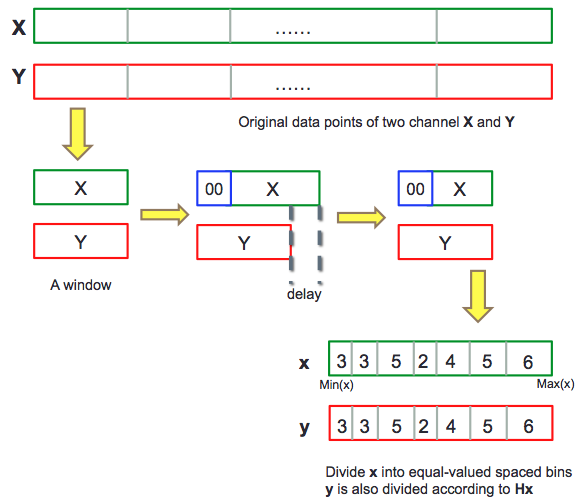
\includegraphics[width=0.45\textwidth]{./images/binsepa.png}
    \caption{An example of separating EEG time series into windows and bins for computing the nonlinear regression curves}
    \label{fig:bin}
\end{figure}
Suppose we have two channels of EEG signals $x$ and $y$, then nonlinear regression analysis provides a measure called \emph{correlation ratio} $\eta^2$, whose estimator is called $h^2$. $\eta^2$ (or $h^2$) gives a statistical measure that describes the dependency of signal $x$ on $y$. Assume the amplitude of signal $y$ is a function of the amplitude of signal $x$. The expectation of $y$ given a value of $x$ is denoted as $\mu_{y|x}$ where:
\begin{equation} \label{eq:regressioncurve}
\mu_{y|x} = \int_{-\infty}^{\infty} y p(y|x) \mathrm{d}y,
\end{equation}
and $\mu_{y|x}$ describes the predicted value of $y$ given $x$. By this definition, we can calculate $\eta^2$, which represents the reduction of variance of $y$ that obtained by predicting $y$ value using $\mu_{y|x}$. $\eta^2$ is expressed as:
\begin{equation} \label{eq:NRAregression}
\eta^2 = \frac{Total \ Variance - Unexplained \ Variance}{Total \ Variance}
\end{equation}
Explained variance is the variance calculated from $y$ according to $\mu_{y|x}$. In this paper, the nonlinear regression analysis algorithm is implemented by fieldtrip toolbox\copyright~\cite{oostenveld2010fieldtrip}. the procedure is depicted in Fig. \ref{fig:bin}).

\subsection{Significance Check}
The significance check is similar for both methods (Grancer causality and Nonlinear Regression Analysis) and is split into two main parts: (1) $p$-value calculation for samples based on theoretical asymptotic null distribution; (2) statistical significance adjusted for \emph{Bonferroni} correction. The rationale behind applying a significance check is to keep only the significant connections. 

The \emph{null hypothesis} $H_0$ is set to "there is no functional connectivity between two channels". In this paper, we assume that the connectivity values emanate from a normal distribution and the $p$-value that rejects the null hypothesis is set to $p=0.05$. The commonly used $F$-statistics is applied for estimating the $p$-value both for Granger Causality and for Nonlinear Regression Analysis.

All the values in functional connectivity maps that passed significance check are kept for feature extraction and classification in later steps. In order to keep the information about the strength of the connections, we use weighted maps. The weights emanate from the original values of the functional connectivity maps (estimated either with Granger causality or with nonlinear regression analysis) that survived the significance check (an example is presented in Fig. \ref{fig:weightednetwork}).

%\begin{Fig.}[!t]
%    \centering
%    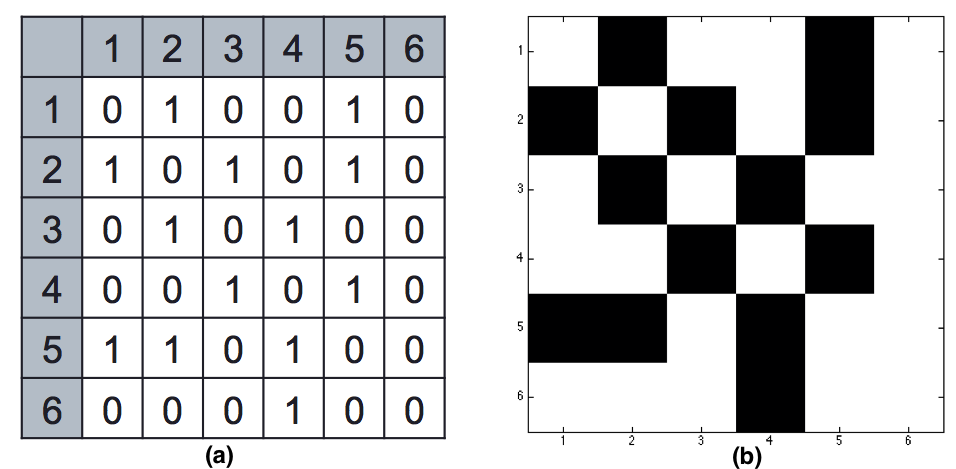
\includegraphics[width=0.45\textwidth]{./images/unweightednetwork.png}
%    \caption{An example of unweighted functional connectivity map construction of size $6 \times 6$. Nodes in (a) with value 1 represents the nodes that passed significance check. (b) is a visual expression of unweighted functional connectivity map.}
%    \label{fig:unweightednetwork}
%\end{Fig.}

\begin{figure}[t]
\centering
%\mbox{
	\leavevmode
\subfigure[]{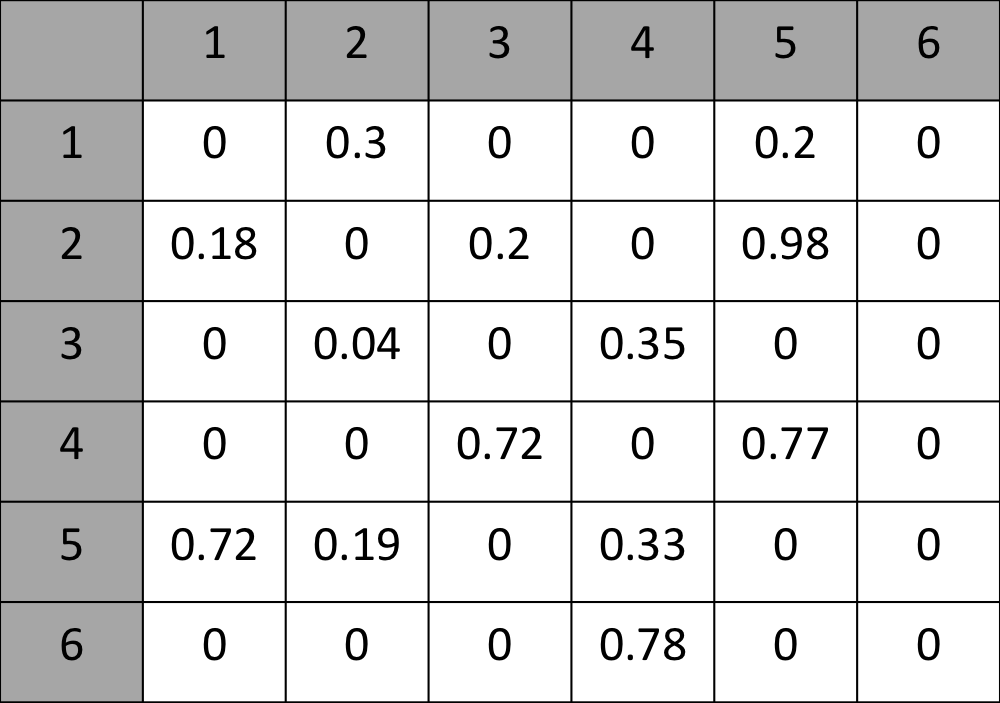
\includegraphics[width=0.48\linewidth]{images/weighted_fcm0.png}}
\subfigure[]{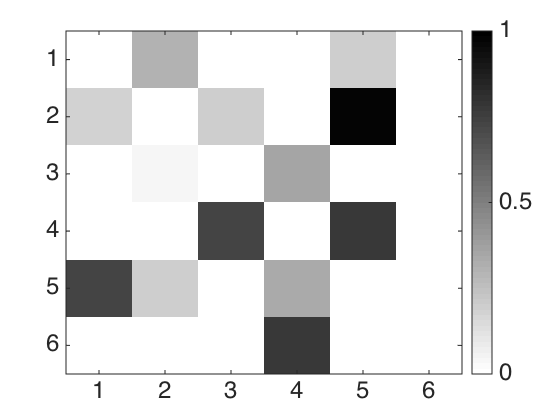
\includegraphics[width=0.48\linewidth]{images/weighted_fcp.png}}
%}
\caption{An example of a weighted functional connectivity map of size $6 \times 6$. In (a) the values represent the weights of the nodes. Each weight corresponds to the value of the underlying functional connectivity map. (b) A visual presentation of the same weighted functional connectivity map.}\label{fig:weightednetwork}
\end{figure}

%\begin{figure}[!t]
%    \centering
%    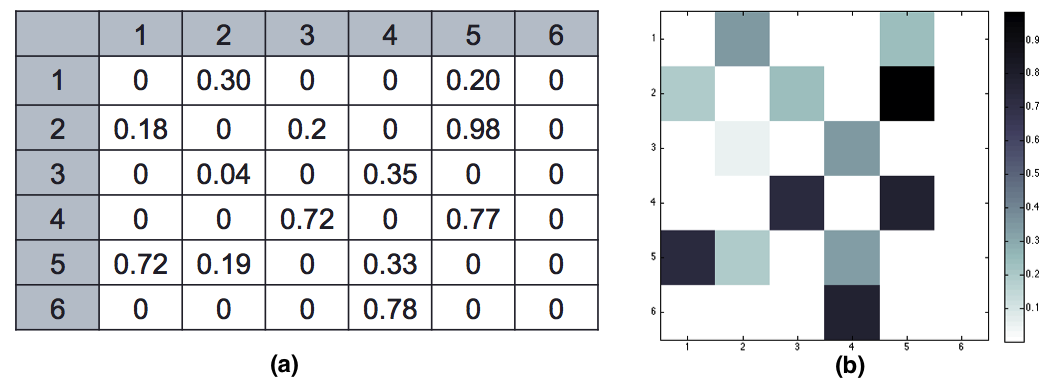
\includegraphics[width=0.45\textwidth]{./images/weightednetwork.png}
%    \caption{An example of a weighted functional connectivity map of size $6 \times 6$. In (a) the values represent the weights of the nodes. Each weight corresponds to the value of the underlying functional connectivity map. (b) A visual presentation of the same weighted functional connectivity map.}
%    \label{fig:weightednetwork}
%\end{figure}

\subsection{Network Feature Extraction}
The functional connectivity maps give us a view of how channels communicate information with each other, thus we can consider this map as a network. Different ways of treating brain networks have been proposed by different groups. For instance, some research groups see the brain as a scale-free network~\cite{eguiluz2005scale}, while others view it as a small-world network~\cite{bassett2006small}. In this section, we introduce two categories of network features, based on the principles of scale-free networks and of small-world networks, namely -- \emph{physical statistics} features for scale-free networks, and \emph{graph theory-based} features for small-world networks.

\subsubsection{Small-World Network Features}
A small-world network consists of nodes that can be reached from every other node with a small number of steps. Different aspects of small-world networks have been studied and here, based on the commonly used features in neural network studies, we introduce four features for analysing the functional connectivity maps which are \emph{characteristic path}, \emph{global efficiency}, \emph{local efficiency} and \emph{clustering coefficient}~\cite{watts1998collective}~\cite{latora2001efficient}.

\emph{Characteristic path} represents the average shortest path of the network. The minimum value is achieved when the network is a complete graph (every pair of distinct vertices is connected by a unique edge). In our case, we can interpret the characteristic path as a feature representing the number of connections in the functional connectivity networks. The more the connections in the functional connectivity network, the smaller the value of the characteristic path, thus the faster the information that is transferred through the network. 

The concept of \emph{global efficiency} of a small-world network is introduced by Latora and Marchiori~\cite{latora2001efficient} and provides a measure of efficient behaviour of the network, by assuming that the network system is parallel (i.e., every vertex sends information concurrently through its edges in the network). The global efficiency of the network is higher when the characteristic path is short. Thus, global efficiency measures how efficiently the vertices exchange information through the network concurrently. Similarly with global efficiency, \emph{local efficiency} is defined as the average efficiency of the subgraphs of the neighbours of a vertex $i$ in the graph (details of computing subgraphs can be referred to~\cite{ullmann1976algorithm}). The subgraphs of $i$ do not contain vertex $i$, hence, the local efficiency can show how efficient the communication is when $i$ is removed from the network. Thus the local efficiency reveals how much the network is fault tolerant. 

Finally, \emph{clustering coefficient} of a network measures the degree to which vertices in a graph tend to cluster together. The overall level of clustering in a network is given by Watts and Strogatz~\cite{watts1998collective} as the average of the local clustering coefficients of all vertices. 

\subsubsection{Scale-Free Network Features}
Although graph theory has been successfully used to describe brain functional connectivity networks, a few studies have shown that brain functional connectivity can also be considered as a scale-free network. An example of a scale-free compared to a random network is presented in Fig. \ref{fig:scalefree}. The number of links $k$ of a node in a scale-free network follows a power law distribution as \eqref{eq:pwlaw}.
\begin{equation} \label{eq:pwlaw}
P(a \ node \ having \ k \ links ) \sim k^{-\lambda}
\end{equation}
where $\lambda$ is a parameter valued in the range $2<\lambda<3$.
Groups of CJ Stam~\cite{stam2004functional} have found that brain functional connectivity network can be viewed as a scale-free network because the connectivity distribution followed a power-law scaling with an exponent close to two.
%, which suggests such functional connectivity network can be considered as a scale-free network topology~\cite{van2008small}. Detailed analysis can also be found in Thivierge's work~\cite{thivierge2014scale}.

\begin{figure}[!t]
    \centering
    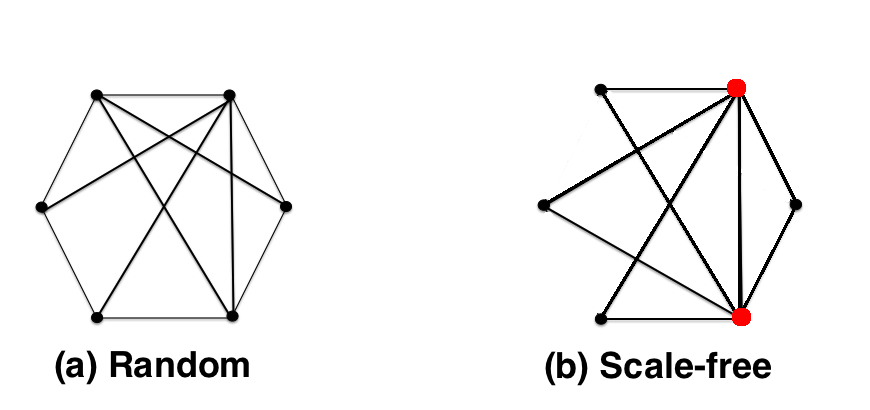
\includegraphics[width=0.4\textwidth]{./images/Scale-free.png}
    \caption{An example of a random network (a) compared with a scale-free network (b) . Red nodes in (b) represent the hubs holding connections in the subgraph.}
    \label{fig:scalefree}
\end{figure}

In information theory, \emph{entropy} plays an important role in measuring uncertainty. Recently, following theoretical and statistical mechanics paradigms, several entropy measures for complexity have been proposed for network structures, and these measures have shown good performance in quantifying the level of organisation encoded in structural features of scale-free networks. It is well known that \emph{Shannon entropy} and \emph{von Neumann entropy} are related to the information present in classical and quantum systems respectively. Both of them can be used to analyse the structural organisation of scale-free networks\cite{anand2009entropy}. 

The amount of \emph{Shannon entropy} has a correlation with the number of network structural constraints. Examples of network constrains include: a) fixed number of links per vertex, b) given degree sequence (a monotonic non-increasing sequence of the degrees of vertices in the graph), and c) community structure (vertices of the network can be easily grouped into sets of vertices such that each set of vertices is densely connected internally). From this point of view, we can conclude that Shannon entropy has a clear interpretation of quantifying the information presented in network structure (Detailed proof can be referred to~\cite{anand2009entropy}). If a network has a smaller Shannon entropy, it will have more constrains on its structure, which shows this network is more optimal. 

\emph{Von Neumann entropy} has been defined by von Neumann for proving the irreversibility of quantum measurement processes. Recently it is also shown that von Neumann entropy can also be applied to network analysis~\cite{passerini2008neumann}. It has been shown that von Neumann entropy is a measure of regularity of networks~\cite{passerini2008neumann}. For a fixed number of edges, regular networks (networks whose vertices have the same number of neighbours) have in general a higher von Neumann entropy. It is also shown that von Neumann entropy depends on the number of connected components, long paths and nontrivial symmetries. With a fixed number of edges, von Neumann entropy is smaller for networks with higher degree of cluster. The mathematical proofs can be found in~\cite{passerini2008neumann} and~\cite{anand2009entropy}.

Thus, to sum up, network-based features including characteristic path, local efficiency, global efficiency, clustering coefficient, Shannon entropy and von Neumann entropy are extracted from the estimated functional connectivity maps for classification purposes. 

\subsection{Classification}

Support vector machine with a \emph{Gaussian radial basis function} kernel is used for classification. The parameter selection of $\sigma$ in RBF kernel is based on cross-validation. In particular, the dataset is split into three parts, namely training, validation and testing. Leave-one-subject-out (LOO) cross-validation is carried out to estimate the parameter $\sigma$. The testing is also carried out in a LOO cross-validation scheme. We tested 13 different values of parameter $\sigma$ ranged from 0.01 to 2. More specifically, the parameter $\sigma$ is selected based on the training and validation using data from 22 subjects, while one subject is left out for testing. The procedure is repeated until all subjects have been left out as test-subjects (i.e., the procedure is repeated 23 times). 

Cohen's Kappa $\kappa$~\cite{uebersax1987diversity}, is a measure of agreement between two viewers, and is calculated to evaluate the classifier's performance. 
%Some researchers consider that Cohen's kappa can be used to evaluate the agreement by chance, i.e. if the viewers are randomly guessing for a decision. 
In our case the two viewers actually correspond to the ground truth and test labels. Cohen's kappa is considered an accurate metric for classification performance and takes into account unbalanced classes (i.e., classes with different number of samples). 


\section{Results and Discussion}

The classification results for the features extracted from the functional connectivity maps are shown in Fig. \ref{fig:kappa}. Higher kappa values indicate better classification performance. A kappa value $k=0$ indicates a random decision. According to Figure \ref{fig:kappa}, a higher classification performance is achieved with Nonlinear Regression Analysis (NRA) compared to Granger's Causality (GC). One-way \emph{Student-t test} was applied to test the significance of non-randomness. The null hypothesis is that the kappa values for each case follow a Student distribution with zero mean. The NRA results sucessfully passed the test with $p<0.05$ (with $\kappa$ value $\mu = 0.06, \sigma = 0.14$, 14 out of 23 subjects have kappa values larger than zero). The null hypothesis is not rejected for the GC case. The higher kappa values from NRA network classifiers indicate that nonlinear patterns occur in the functional connectivity of neural assemblies, who able to discriminate between pleasantness and unpleasantness during olfactory perceptions. 

\begin{figure}[t]
    \centering
    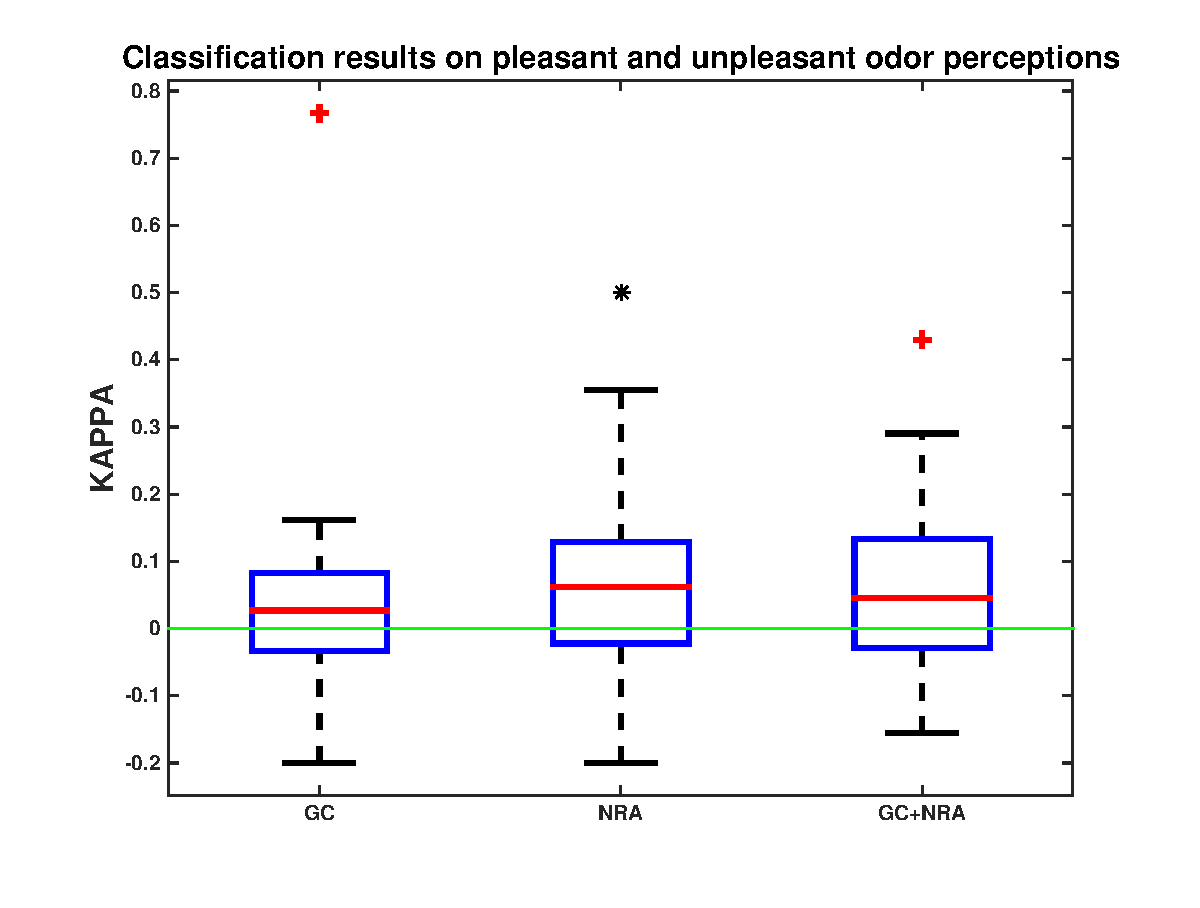
\includegraphics[width=0.45\textwidth]{./images/kappa.eps}
    \caption{Cohen's Kappa results boxplots. On each box, the central (red) line represents the median value, the upside and downside edges represent the 25th and 75th percentiles, and the red crosses represent outliers. The green line represents the random decision, $Kappa=0$. GC refers to the kappa values estimated for features extracted from the functional connectivity maps estimated using Granger Causality. NRA refers to the kappa values estimated for features extracted from the maps estimated using Nonlinear Regression Analysis. GC+NRA refers to the kappa values estimated using features both from Granger Causality and from Nonlinear Regression Analysis.}
    \label{fig:kappa}
\end{figure}

%%%%%%%%%%%%%%%%%%%%%%%%%%%%%%%%%%%%%%%%%%%%%%%%%%%%%%%%%%%%%%%%%%%%%%%%%%%%%%
%%                             TABLE 1
%%%%%%%%%%%%%%%%%%%%%%%%%%%%%%%%%%%%%%%%%%%%%%%%%%%%%%%%%%%%%%%%%%%%%%%%%%%%%%
\begin{table}[ht]
\caption{Kappa descriptives for each classification scenario. Min stands for minimum kappa value, max for maximum kappa value, and SD for standard deviation. One asterisk indicates significance with $p<0.05$, and two asterisks with $p<0.01$.}\label{Table1}
\centering % for placing the table in the middle of the page
{\begin{tabular}{|l|c|c|c|c|}
\hline
\toprule
 \textbf{Features} & \textbf{Min} & \textbf{Max} & \textbf{Mean} & \textbf{SD} \\
\hline
\toprule
\textbf{GC} & -0.2 & 0.77 & 0.07 & 0.23 \\
\hline
\toprule
 \textbf{NRA*} & -0.2 & 0.19 & 0.06 & 0.14 \\
\hline
\toprule
\textbf{GC+NRA*} & -0.07 & 0.18 & 0.05 & 0.08  \\
\hline
\toprule
\textbf{NRA(Characteristic path**)} & -0.1 & 0.45 & 0.096 & 0.15 \\
\hline
\toprule
\textbf{NRA(Local efficiency**)} & -0.14 & 0.37 & 0.09 & 0.14 \\
\hline
\toprule
\textbf{NRA(Global efficiency**)} & -0.17 & 0.5 & 0.11 & 0.17 \\
\hline
\toprule
 \textbf{NRA(Clustering coefficient**)} & -0.15 & 0.5 & 0.11 & 0.16 \\
\hline
\toprule
\textbf{NRA(Shannon entropy)} & -0.13 & 0.34 & 0.07 & 0.12 \\
\hline
\toprule
\textbf{NRA(von Neumann entropy)} & -0.13 & 0.3 & 0.01 & 0.12 \\
\bottomrule
\end{tabular}}
%\begin{tabnote}
%SD indicates Significant Differences (with $p<0.01$), whereas NS indicates No Significant differences ($p>0.05$).
%\end{tabnote}
\end{table}
%%%%%%%%%%%%%%%%%%%%%%%%%%%%%%%%%%%%%%%%%%%%%%%%%%%%%%%%%%%%%%%%%%%%%%%%%%%%%%

%In order to investigate the classification performance of the two feature-categories, namely the small-world network features and the free-scale network features, a SVM classifier is trained and tested as previously, for each feature-category. The results are presented in Table \label{Table1}. In order to investigate if each feature-category leads to significantly non-random kappa values, a one-way \emph{Student-t test} is applied as previously. The results reveal that the small-world network features lead to a significantly non-random performance, whereas this is not the case for the free-scale network features. This finding indicates that odor pleasantness perception can be depicted in small-world network features extracted from the functional connectivity across neural assemblies which is estimated using Nonlinear Regression Analysis. 
%
%
%Finally, in order to further explore which individual feature increases the classification performance, the same analysis as previously is carried out for each feature. The results are also presented in Table \lref{Table1}. According to this table, all small-world network features lead to a similar classification performance, which is significantly non-random ($p<0.01$). 
The most representative kappa descriptives are summarised in Table \ref{Table1}. \textbf{GC} represents the network features (both small-world and scale-free types) extracted from Linear Granger Causality functional connectivity network. \textbf{NRA} represents the network features (both small-world and scale-free types) extracted from Nonlinear Regression Analysis functional connectivity network. \textbf{GC+NRA} represents the combined network features from both functional connectivity networks. Since the NRA network gives a better kappa performance, we further investigated the classification performance of each single network feature of the NRA functional connectivity network, using the same scenario of classification and statistical tests as described in previous sections. The results reveal that the small-world network features (characteristic path, local efficiency, global efficiency and clustering coefficient) have a better classification performance compared to scale-free network features. This result indicates that odor pleasantness perception can be depicted in small-world network features extracted from the functional connectivity across neural assemblies which is estimated using Nonlinear Regression Analysis. 

Additionally, free-scale networks are known for their property of self-similarity in finer scales. However, in our case free-scale network features did not lead to significantly non-random results, indicating that self-similar properties of functional connectivity maps may not be responsible for odor pleasantness discrimination. 

However, the best obtained accuracy ($0.11 \pm 0.17$), although significantly non-random, is not very high. Compared with previous study on olfactory pleasantness perception using other methods such as power spectral density~\cite{kroupi2014eeg}, our results are not outstanding. We expect that by integrating information from the brain functional connectivity with commonly used features for odor pleasantness perception (such as power spectral density features), the classification performance can be improved. 

This work in analyzing network features from functional connectivity networks in general can have a great impact in affective computing. The method we had proposed in this paper can help revealing additional knowledge about how information flows during underlying emotional processes. Due to the limitations of research on odors (still many questions open regarding exposition time, etc.), it would be very interesting to further explore if similar patterns occur and if the classification performance is increased using more conventional affective stimuli, such as video and audio.   


%Although the significant kappa result have a $p-values$ less than 0.05, some of the $p-values$ are still very close to 0.05, indicating that the results are not that good anyway.The low classification accuracy may due to many reasons: the size of functional connectivity map may play a crucial rule in classification -- the 216-channel functional connectivity maps may provide too much redundant information in classification. New features of functional connectivity maps should also be proposed and used for classification. Since we only used network-based features in this paper, other features as power spectral density or time-frequency analysis may also be used in combination for classification. Another improvement for getting better classification results could be done in the experiment design. Based on the experiment protocol and preprocessing of raw EEG signal, 6 seconds of each trial of EEG signal are kept fro investigating the pleasantness from odors. This time duration could be cut shorter (because 6 seconds might be to much for decision making) or extended longer (or because 6 seconds might be not enough to make the decision). Nevertheless, this paper is not targeting to replace existing methods for affective computing on emotions, but to propose a new direction for affective computing. 

\section{Conclusion}
The concept of functional connectivity maps has been used to study the brain activity but it has not yet been used for classifying odor pleasantness perception. In this paper, we compared different methods of estimating functional connectivity from EEG signals for 23 subjects in order to classify pleasant and unpleasant odors. By considering the connectivity maps as networks, physical statistics and graph theory based features were extracted and used in SVM classifiers. The best classification accuracy based on Cohen's Kappa was achieved using nonlinear regression analysis and small-world network features to estimate the connectivity maps. The results indicated that nonlinear patterns occur in the connectivity maps during hedonic olfactory perception, able to classify odor pleasantness perception in a significantly non-random way.  







% trigger a \newpage just before the given reference
% number - used to balance the columns on the last page
% adjust value as needed - may need to be readjusted if
% the document is modified later
%\IEEEtriggeratref{8}
% The "triggered" command can be changed if desired:
%\IEEEtriggercmd{\enlargethispage{-5in}}

% references section

% can use a bibliography generated by BibTeX as a .bbl file
% BibTeX documentation can be easily obtained at:
% http://www.ctan.org/tex-archive/biblio/bibtex/contrib/doc/
% The IEEEtran BibTeX style support page is at:
% http://www.michaelshell.org/tex/ieeetran/bibtex/
%\bibliographystyle{IEEEtran}
% argument is your BibTeX string definitions and bibliography database(s)
%\bibliography{IEEEabrv,../bib/paper}
%
% <OR> manually copy in the resultant .bbl file
% set second argument of \begin to the number of references
% (used to reserve space for the reference number labels box)
%\begin{thebibliography}{1}

%\bibitem{IEEEhowto:kopka}
%H.~Kopka and P.~W. Daly, \emph{A Guide to \LaTeX}, 3rd~ed.\hskip 1em plus
%  0.5em minus 0.4em\relax Harlow, England: Addison-Wesley, 1999.

%\end{thebibliography}
\scriptsize
\bibliographystyle{IEEEtran}
\bibliography{ref.bib}



% that's all folks
\end{document}


